\section{Auswertung}
\label{sec:Auswertung}
\subsection{Magnetfeld}
Wie in Abschnitt \ref{sec:Durchführung} beschrieben, wird zunächst die Stärke des Magnetfeldes $B$ in Abhängigkeit des angelegten Stroms $I$ bestimmt.
Die aufgenommenen Messwerte sind in der \autoref{tab:Magnetfeld} zu sehen.

\begin{table}
    \centering
    \caption{Magnetfeldstärke $B$ in Abhängigkeit des an den Spulen angelegten Stroms $I$}
    \sisetup{table-format=3.1}
    \begin{tabular}{S[table-format=3.1] S S S S}
        \toprule
        $I / \si{\ampere}$ & $B / \si{\milli\tesla}$ &$I / \si{\ampere}$ & $B / \si{\milli\tesla}$ \\
        \midrule
        0   &     7 &   3   & 280 \\
        0.5 &    51 &   3.5 & 325 \\
        1   &    97 &   4   & 367 \\
        1.5 &   142 &   4.5 & 407 \\
        2   &   188 &   5   & 443 \\
        2.5 &   235 &       &     \\
        \bottomrule
    \end{tabular}
    \label{tab:Magnetfeld}
\end{table}
Die aufgenommenen Werte werden in \autoref{fig:Magnetfeld} gegeneinander aufgetragen.
Dabei wird die Abbildung mit dem Python Paket 'matplotlib' \cite{matplotlib} erstellt.
Zudem wird eine Ausgleichsrechung für die Messwerte durchgeführt.
Die Rechung wurde mit dem Python Paket 'scipy' \cite{scipy} nach der Funktion
\begin{equation*}
    f(x) = ax^3 +bx^2+cx+d
\end{equation*}
durchgeführt und ergibt für die Koeffizienten:
\begin{align*}
    a =& \SI{-0.766}{\milli\tesla}   \\
    b =& \SI{4.207}{\milli\tesla} \\
    c =& \SI{85.318}{\milli\tesla} \\
    d =& \SI{7.314}{\milli\tesla} \\
\end{align*}

\begin{figure}
    \centering
    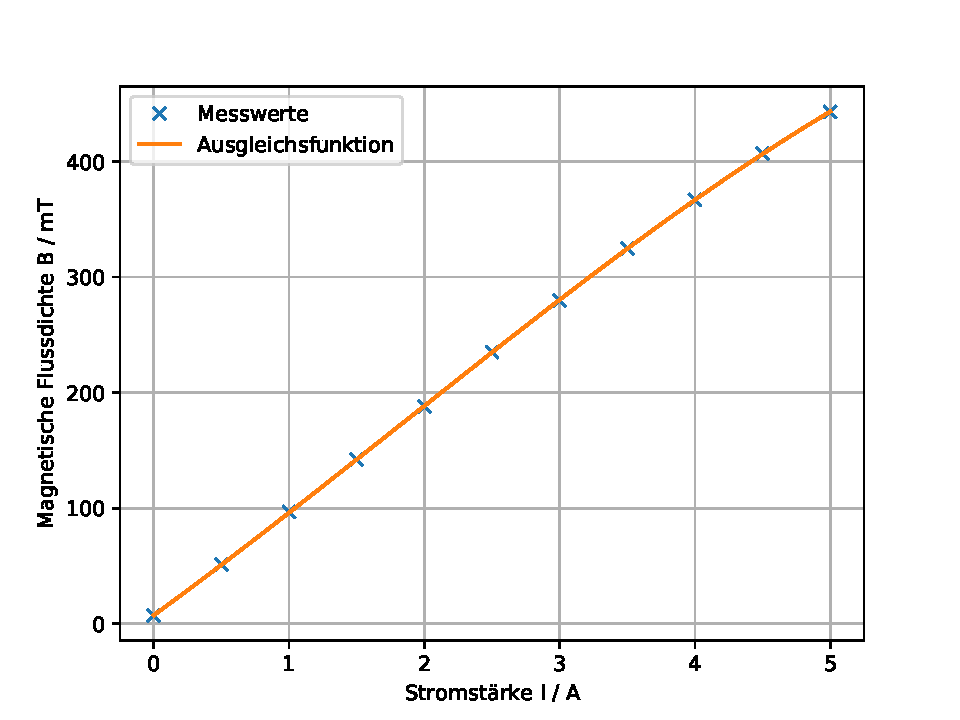
\includegraphics[width=0.75\textwidth]{content/data/magnetfeld.pdf}
    \caption{Der angelegte Strom $I \, \text{in} \, \si{\ampere}$ aufgetragen gegen die gemessene Magnetfeldstärke $B \, \text{in} \, \si{\milli\tesla}$.}
    \label{fig:Magnetfeld}
\end{figure}

\subsection{Blaue Spektrallinie}

\subsubsection{\boldmath \texorpdfstring{$\pi$}{pi}-Polarisiertes Licht}
Zunächst wird wie im Abschnitt \ref{sec:Durchführung} beschrieben, die Änderung der blauen Spektrallinie im Magnetfeld aufgenommen.
Das Bild der Aufspaltung für das $\pi -$Polarisierte Licht ist dabei in \autoref{fig:pi-blau} zu sehen.
In der Grafik wird die Blauen Spektrallinien ohne Einfluss durch ein Magnetfeld und die Spektrallinie des $\pi -$Polarisierten Lichts im Magnetfeld übereinander gelegt.
Oben befindet sich dabei das Licht welches durch das Magnetfeld beeinflusst wird und unten das Licht welches nur durch durch das Prisma gebrochen wird.
\begin{figure}
    \centering
    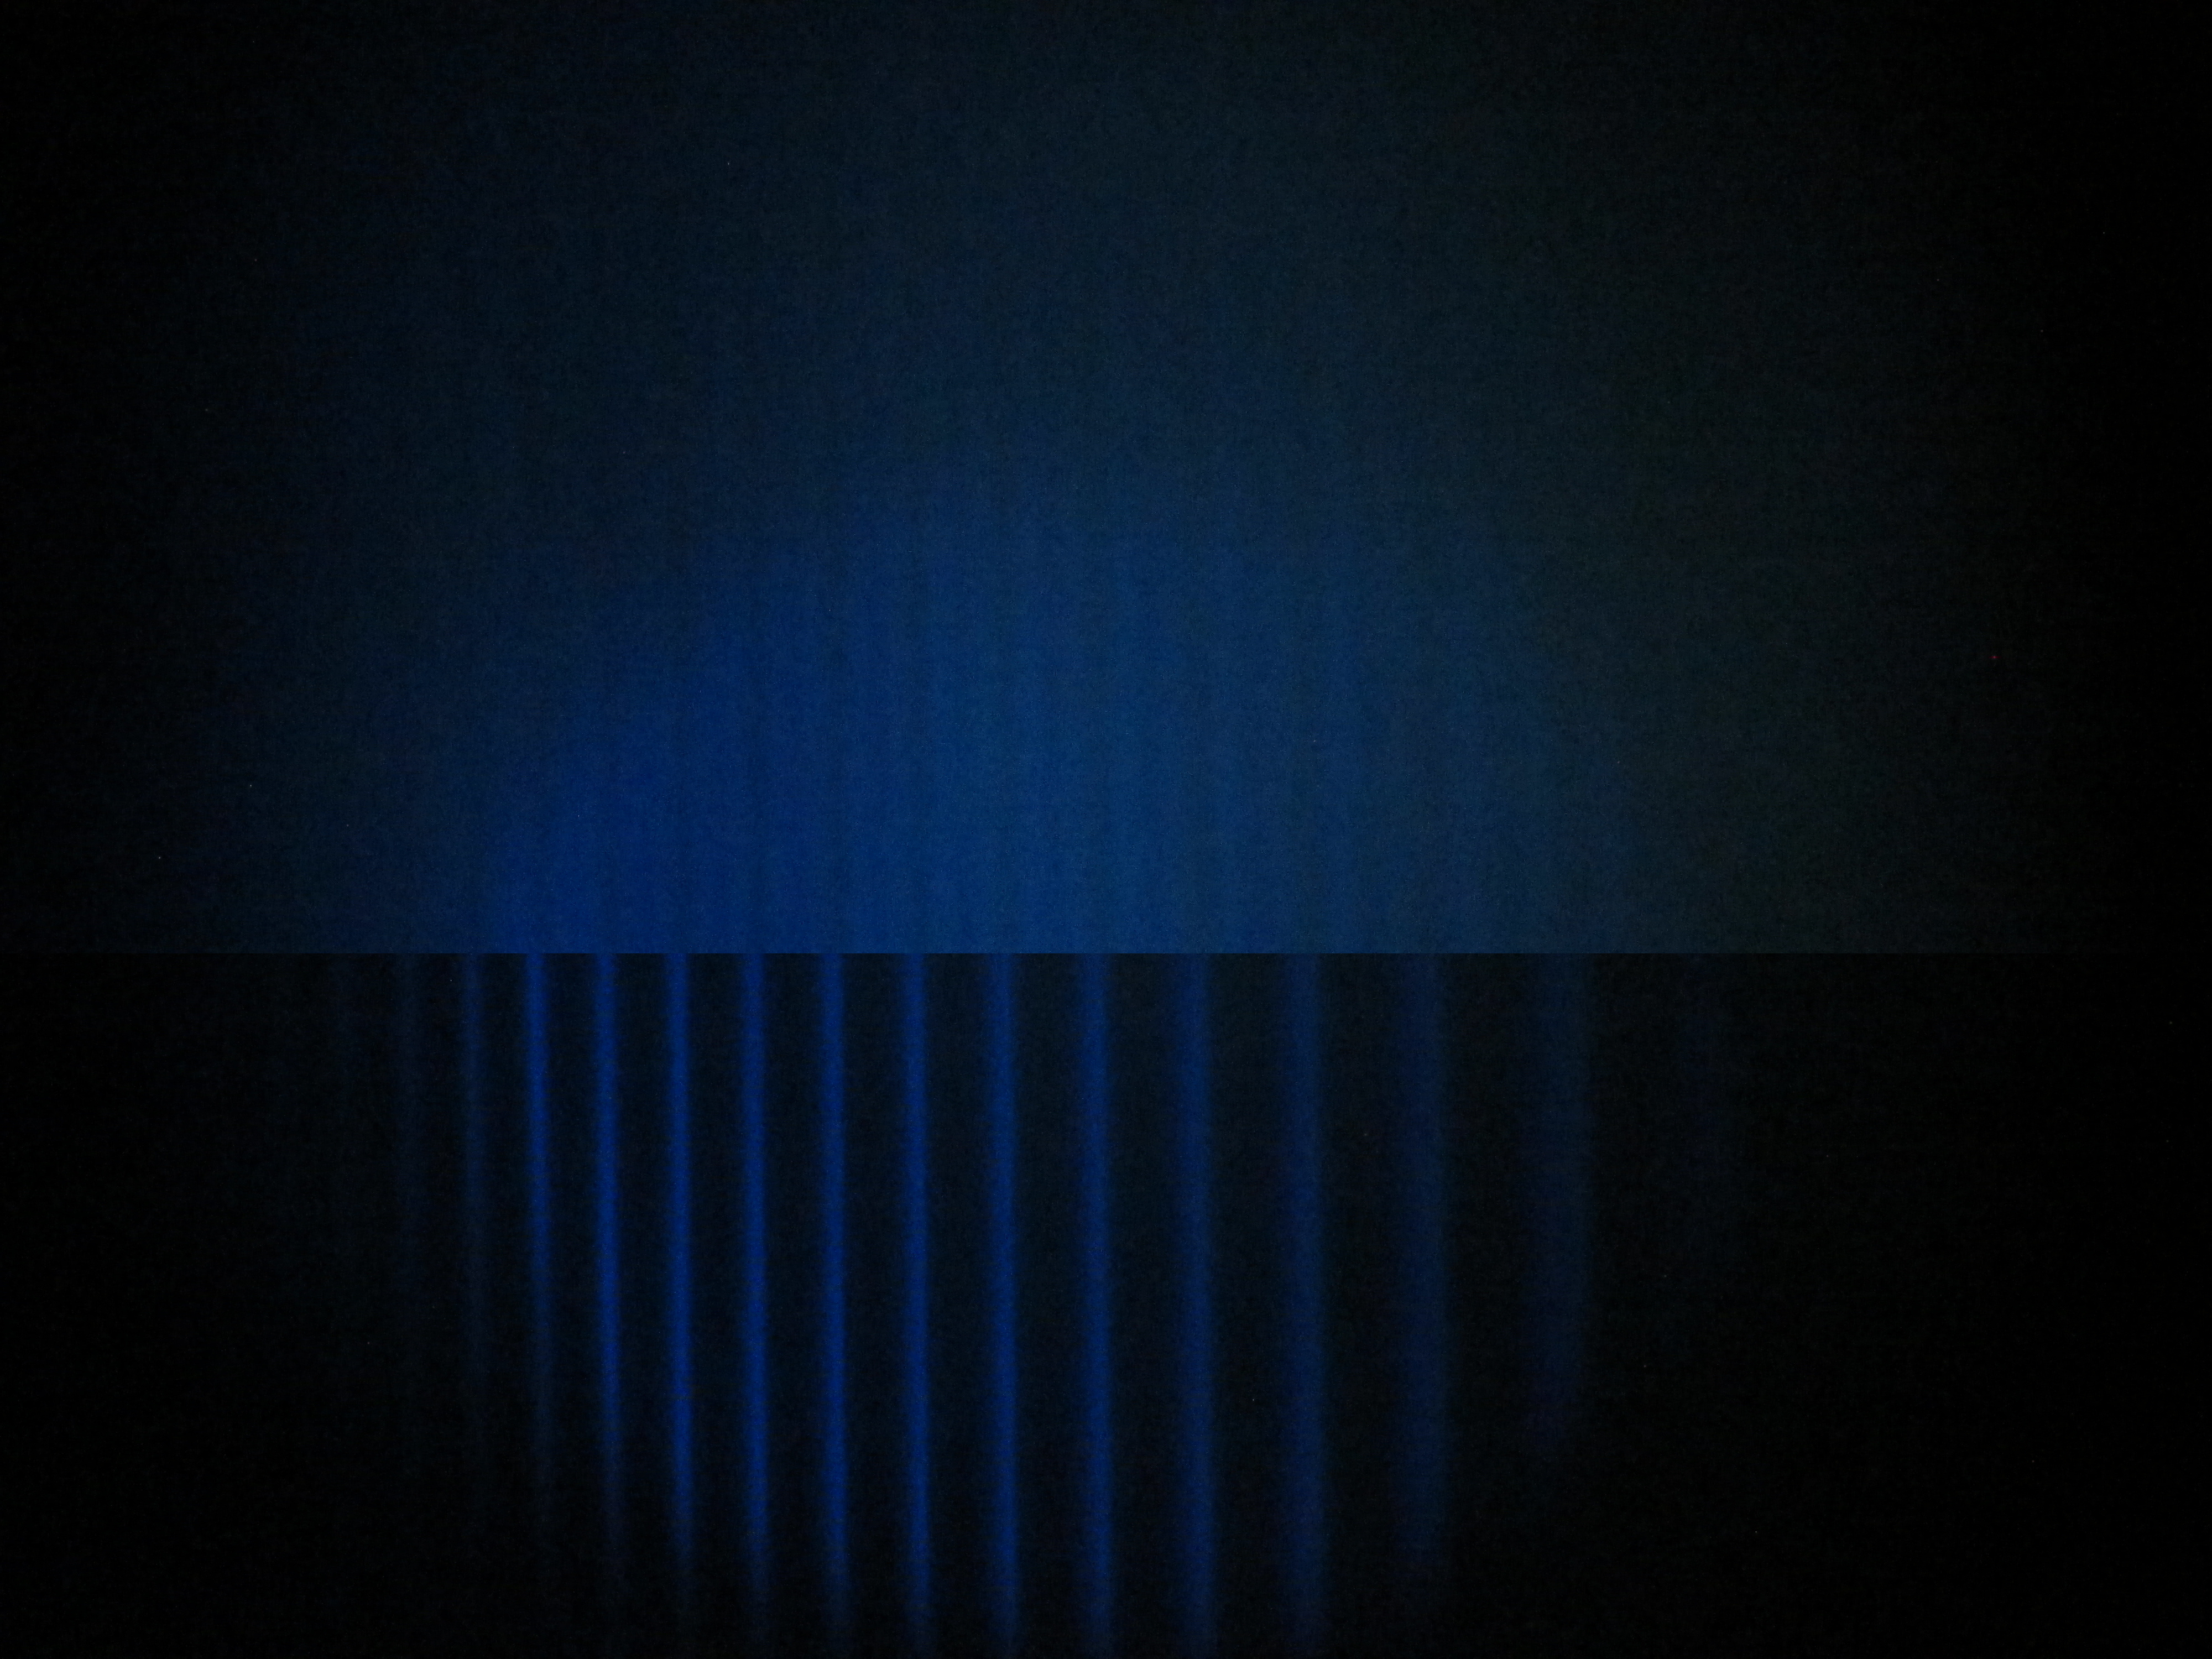
\includegraphics[width=0.75\textwidth]{content/data/Blau_0_pi_uebernander.JPG}
    \caption{Im oberen Teil des Bilder ist das $\pi -$Polarisierte Licht unter Einfluss des Zeeman-Effekts zu sehen. Im unteren Teil ist die blaue Spektrallinie der Lampe ohne Magnetfeld zum Vergleich zu sehen.}
    \label{fig:pi-blau}
\end{figure}
Zur Messung der Wellenlängenverschiebung werden nun die Abstände zwischen Maxima und Maxima der unbeeinflussten Spektrallinien $\Delta s$
und die Abstände zwischen den Anfängen der Maxima der durch den Zeeman-Effekt beeinflussten Maxima $\delta s$ gemessen.
Die Längen werden dabei in Anzahl von Pixeln gemessen und sind in der \autoref{tab:blau-pi} zu finden.
Um die Messwerte zu visualisieren werden die Werte in einem Plot in \autoref{subfig:blau_pi_mess} aufgetragen.
In der linken Grafik sind dabei die Messwerte $\Delta s$ und $\delta s$ zu sehen.
In der \autoref{subfig:blau_pi_versch} dagegen die berechnete Wellenlängenverschiebung $\delta \lambda$.

\begin{table}
    \centering
    \caption{Die Abstände der Maxima der Spektrallinien in Anzahl von Pixel.
    $\Delta s$ gibt dabei die unbeeinflussten Abstände und $\delta s$ die durch den Zeeman-Effekt beeinflussten Abstände, des $\pi -$ Polarisirtem Lichts an.}
    \begin{tabular}{cccc}
        \toprule
        Ordnung & $\Delta s \, /$ Pixel  & $\delta s \, /$ Pixel & $\delta \lambda \, / \, \si{\nano\meter}$  \\
        \midrule
        1  &    270 &   56  & $\SI{0.00281(25)}{}$ \\
        2  &    270 &   54  & $\SI{0.00271(25)}{}$ \\
        3  &    224 &   52  & $\SI{0.00315(31)}{}$ \\
        4  &    206 &   54  & $\SI{0.00356(34)}{}$ \\
        5  &    190 &   44  & $\SI{0.00314(36)}{}$ \\
        6  &    182 &   44  & $\SI{0.00328(38)}{}$ \\
        7  &    178 &   44  & $\SI{0.00336(39)}{}$ \\
        8  &    165 &   40  & $\SI{0.00329(42)}{}$ \\
        9  &    150 &   36  & $\SI{0.00326(46)}{}$ \\
        10 &    145 &   36  & $\SI{0.00337(48)}{}$ \\
        11 &    142 &   34  & $\SI{0.00325(49)}{}$ \\
        \bottomrule
    \end{tabular}
    \label{tab:blau-pi}
\end{table}

\begin{figure}
    \caption{Links die Messwerte $\Delta s$ und $\delta s$ gegen die Ordnung geplottet und rechts die berechnete Wellenlängenverschiebung gegen die Ordnung aufgetragen.}
    \begin{subfigure}{0.48\textwidth}
        \centering
        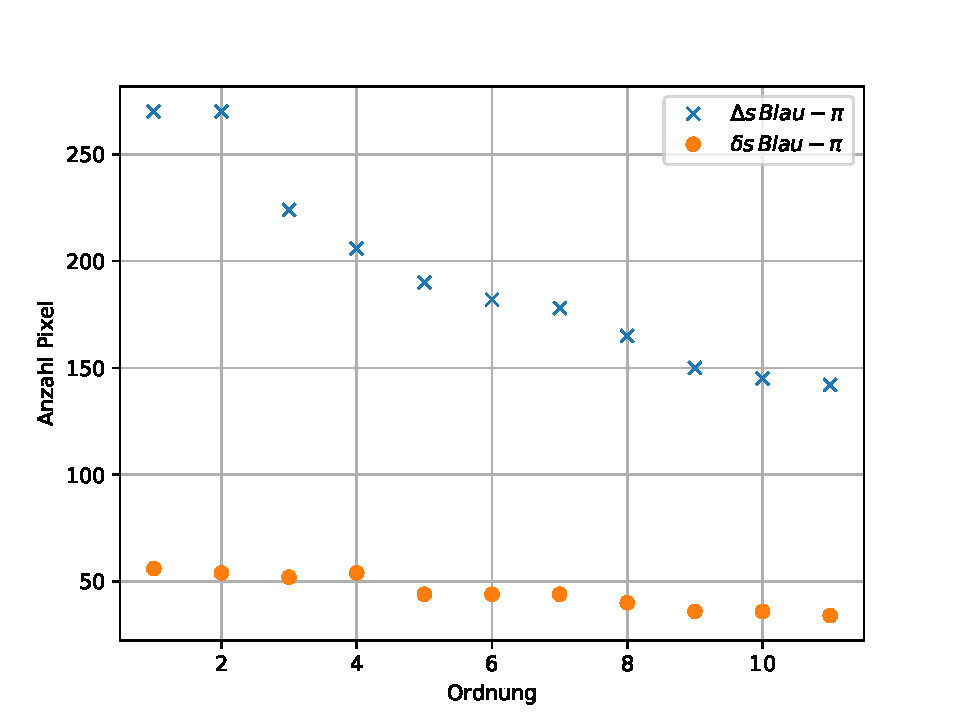
\includegraphics[height=5cm]{content/data/blau_pi_messwerte.pdf}
        \caption{Messwerte $\Delta s$ und $\delta s$ in Anzahl von Pixeln gegen die Ordnung aufgetragen.}
        \label{subfig:blau_pi_mess}
    \end{subfigure}
    \hfill
    \begin{subfigure}{0.48\textwidth}
        \centering
        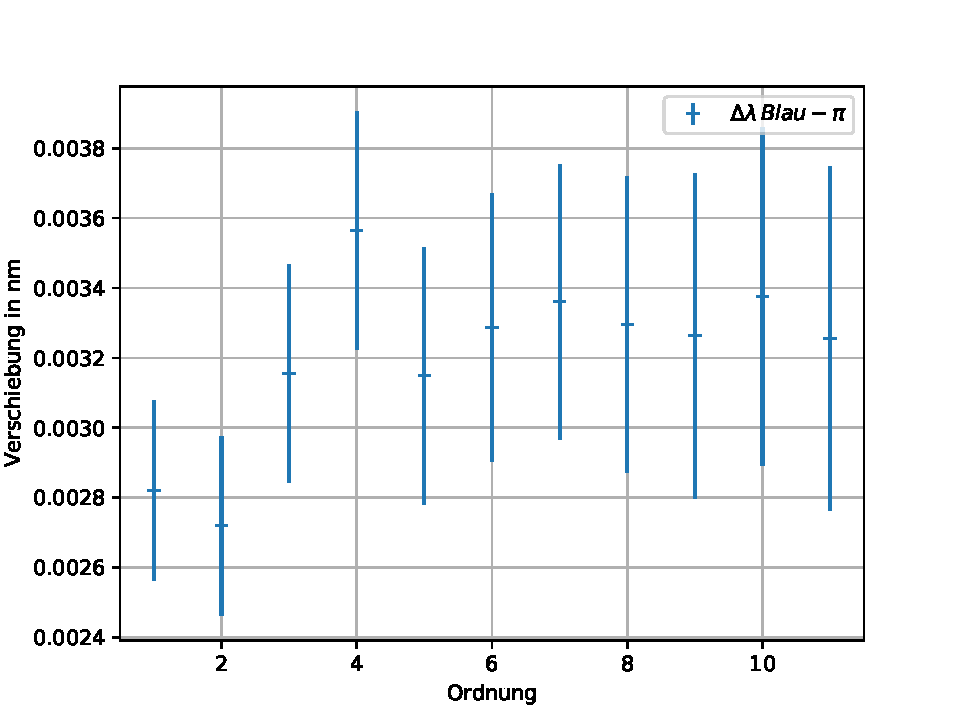
\includegraphics[height=5cm]{content/data/blau_pi_verschiebung.pdf}
        \caption{Die berechnete Wellenlängenverschiebung in $\si{\nano\meter}$ in Abhängigkeit von der Ordnung.}
        \label{subfig:blau_pi_versch}
    \end{subfigure}
    \label{fig:blau_pi_mess_versch}
\end{figure}

Um nun die Wellenlängenverschiebung zu berechnen wird die Formel
\begin{equation}
    \delta \lambda = \frac{\delta s \Delta \lambda _\text{D}}{2\Delta s}
   \label{eq:Wellenlaengenverschiebung}
\end{equation}
mit dem Dispersionsgebiet
\begin{equation*}
    \Delta \lambda _\text{D} = \frac{\lambda^2}{2d\sqrt{n^2-1}}
\end{equation*}
genutzt. 
\FloatBarrier
Die Formel wurde der Quelle \cite[4]{anleitung} entnommen.
Zudem wird ein systematischer Fehler von $\pm 5$ Pixeln angenommen, da die Maxima der Spektrallinie im Programm \cite{paint3d} abgeschätzt worden sind.
Zur Berechung der Fehler der Wellenlängenverschiebung wird das Python Paket \cite{uncertainties} genutzt.
Dieses nutzt zur Berechung der Fehlerfortpflanzung die Formel
\begin{equation}
    F(\delta \lambda) = \frac{1}{2} \Delta \lambda _\text{D} \sqrt{\left (\frac{1}{\Delta s} F(\delta s) \right)^2 + \left ( \frac{\delta s}{\Delta s^2} F(\delta s) \right )^2}
    \label{eq:fehler_Wellenlaengenverschiebung}
\end{equation}
Die berechneteten Werte für die Wellenlängenverschiebung sind in \autoref{tab:blau-pi} zu finden.
Es wird über alle Werte der Wellenlängenverschiebung gemittelt, daraus ergibt sich der Wert

\begin{align*}
    \delta \lambda _\text{$\pi$-blau} = & \SI{0.00316(011)}{\nano\meter} \, . \\
\end{align*}

\subsubsection{\boldmath\texorpdfstring{$\sigma$}{sigma} -Polarisiertes Licht}

%Die selben Berechungen wurden für die Messwerte der $\sigma -$Spektrallinien des Blauen Lichts durchgeführt.
Die Aufspaltung der Maxima des Blauen Licht welches $\sigma -$Polarisiert ist, ist in \autoref{fig:sigma-blau} zu sehen.

\begin{figure}
    \centering
    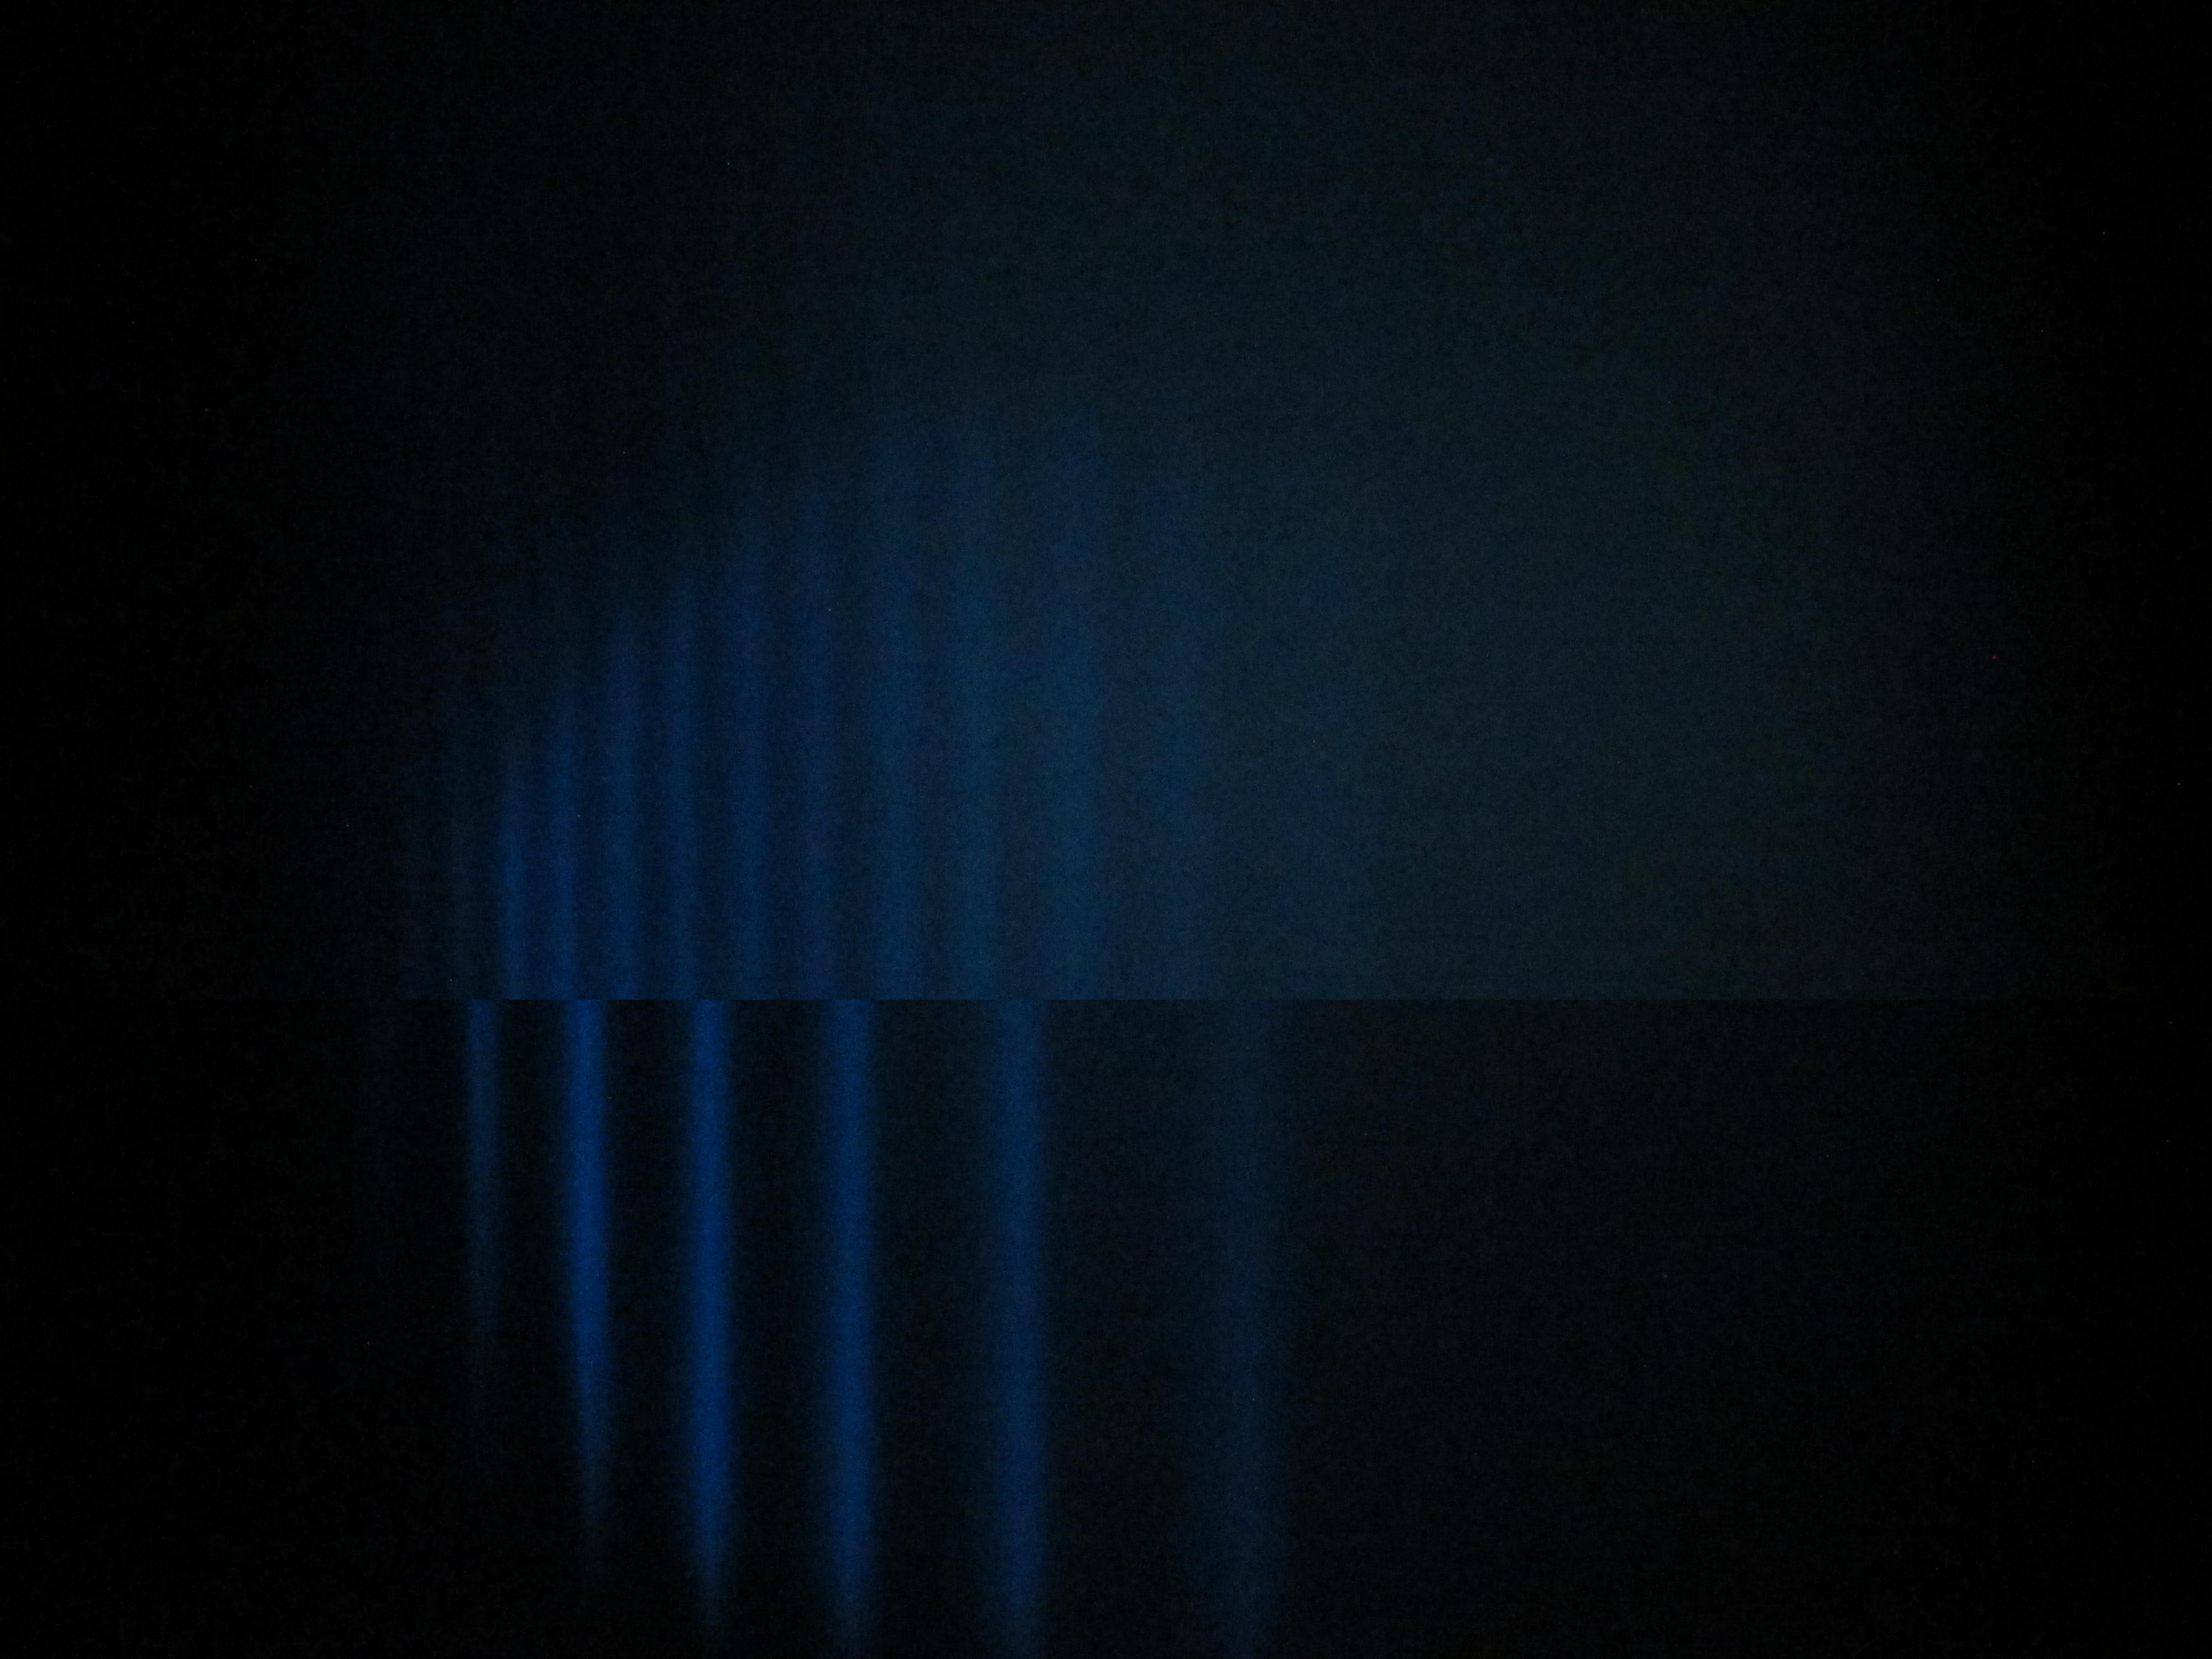
\includegraphics[width=0.75\textwidth]{content/data/Blue_sigma_0_uebernander.JPG}
    \caption{Im oberen Teil des Bilds ist das $\sigma -$Polarisierte Licht unter Einfluss des Zeeman-Effekts zu sehen. Im unteren Teil befindet sich zum Vergleich die blaue Spektrallinie der Lampe ohne Magnetfeld.}
    \label{fig:sigma-blau}
\end{figure}

Zur Bestimmung der Wellenlängenverschiebung wird wie beim $\pi -$Polarisiertem Licht zunächst $\Delta s$ und $\delta s$ gemessen.
Die gemessenen Werte sind in \autoref{tab:blau-sigma} zu sehen.
In \autoref{subfig:blau_sigma_mess} werden die Messwerte $\Delta s$ und $\delta s$ gegen die Ordnung aufgetragen.
In der \autoref{subfig:blau_sigma_versch} wird die Wellenlängenverschiebung $\delta \lambda$ in $\si{\nano\meter}$ gegen die Ordnung geplottet. 

\begin{table}
    \centering
    \caption{$\Delta s$ der blauen Spektrallinie und $\delta s$ des $\sigma -$Polarisiertem Lichts.}
    \begin{tabular}{cccc}
        \toprule
        Ordnung & $\Delta s \, / $ Pixel & $\delta s \, / $ Pixel & $\delta \lambda \, / \,\si{\nano\meter}$ \\
        \midrule
        1   &   270  &    130   & $\SI{0.00654(27)}{}$   \\
        2   &   264  &    130   & $\SI{0.00669(28)}{}$   \\
        3   &   227  &    109   & $\SI{0.00652(32)}{}$   \\
        4   &   200  &    100   & $\SI{0.00679(79)}{}$   \\
        5   &   176  &    91    & $\SI{0.00702(47)}{}$   \\
        6   &   182  &    91    & $\SI{0.00679(17)}{}$   \\
        7   &   164  &    80    & $\SI{0.00663(61)}{}$   \\
        8   &   161  &    70    & $\SI{0.00591(03)}{}$   \\
        9   &   150  &    55    & $\SI{0.00498(26)}{}$   \\
        10  &   133  &    45    & $\SI{0.00459(39)}{}$   \\
        11  &   130  &    38    & $\SI{0.00397(47)}{}$   \\
        \bottomrule
    \end{tabular}
    \label{tab:blau-sigma}
\end{table}

\begin{figure}
    \caption{Links die Messwerte $\Delta s$ und $\delta s$ gegen die Ordnung geplottet und rechts die berechnete Wellenlängenverschiebung gegen die Ordnung aufgetragen.}
    \begin{subfigure}{0.48\textwidth}
        \centering
        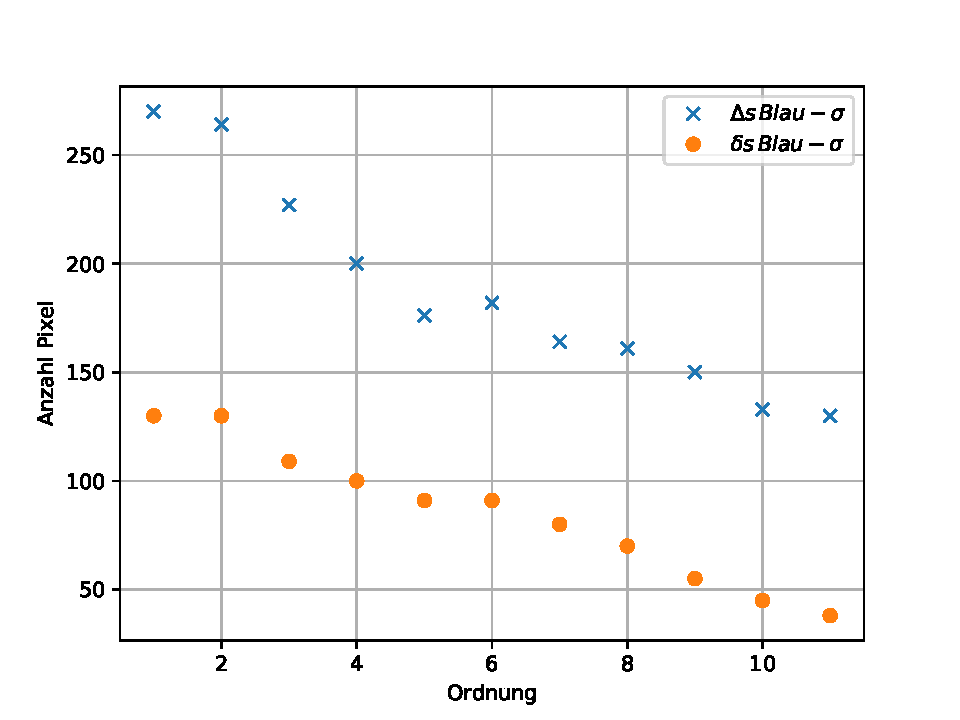
\includegraphics[height=5cm]{content/data/blau_sigma_messwerte.pdf}
        \caption{Messwerte $\Delta s$ und $\delta s$ in Anzahl von Pixeln gegen die Ordnung aufgetragen.}
        \label{subfig:blau_sigma_mess}
    \end{subfigure}
    \hfill
    \begin{subfigure}{0.48\textwidth}
        \centering
        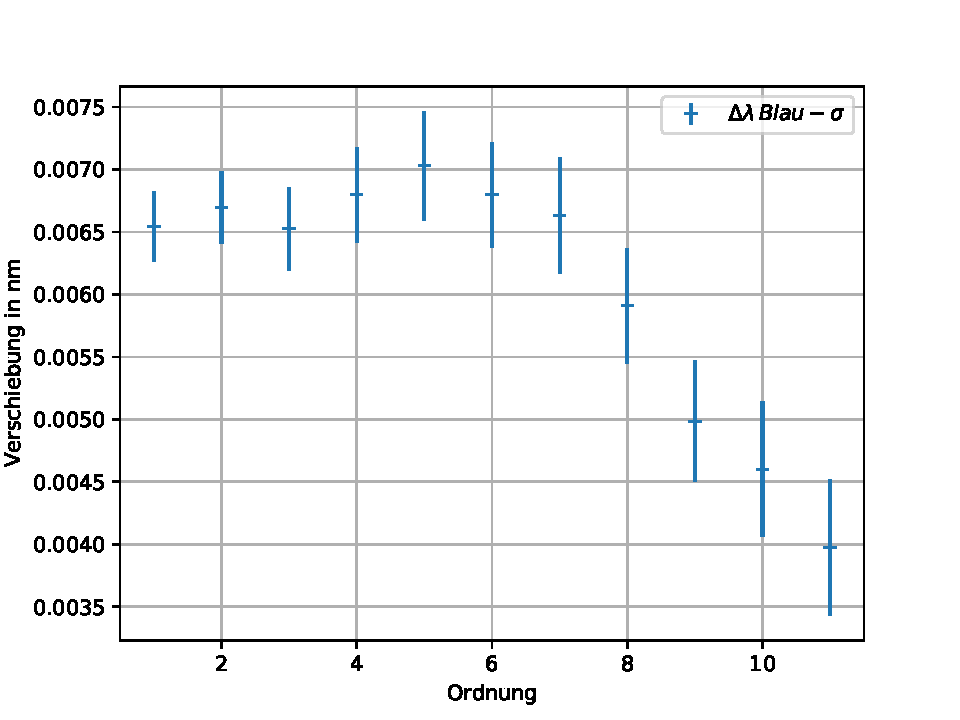
\includegraphics[height=5cm]{content/data/blau_sigma_verschiebung.pdf}
        \caption{Die berechnete Wellenlängenverschiebung in $\si{\nano\meter}$ in Abhängigkeit von der Ordnung.}
        \label{subfig:blau_sigma_versch}
    \end{subfigure}
    \label{fig:blau_sigma_mess_versch}
\end{figure}
\FloatBarrier
Mit den Werte $\Delta s$ und $\delta s$ wird nun die Wellenlängenverschiebung $\delta \lambda$ berechnet, diese ist ebenfalls in der \autoref{tab:blau-sigma} zu sehen.
Zu Berechnung der Wellenlängenverschiebung wird Gleichung \eqref{eq:Wellenlaengenverschiebung} genutzt.
Dabei wird ein systematischer Fehler von $\pm 5$ Pixeln angenommen. 
Hier wird der Fehler nach Gleichung \eqref{eq:fehler_Wellenlaengenverschiebung} bestimmt.
Die Mittlung über alle Wellenlängenverschiebung des $\sigma -$Polarisiertem Lichts ergibt
\begin{align*}
    \delta \lambda _\text{$\sigma$ -blau} =& \SI{0.00621(012)}{\nano\meter} \, .
\end{align*}
\FloatBarrier
\subsection{Rote Spektrallinie}
\subsubsection{\boldmath\texorpdfstring{$\sigma$}{sigma}-Polarisiertes Licht}
Zuletzt wird die Aufspaltung von rotem Licht welches $\sigma -$Polarisiert ist aufgenommen.
Die Aufspaltung ist in der \autoref{fig:rot-sigma} zu erkennen.

\begin{figure}
    \centering
    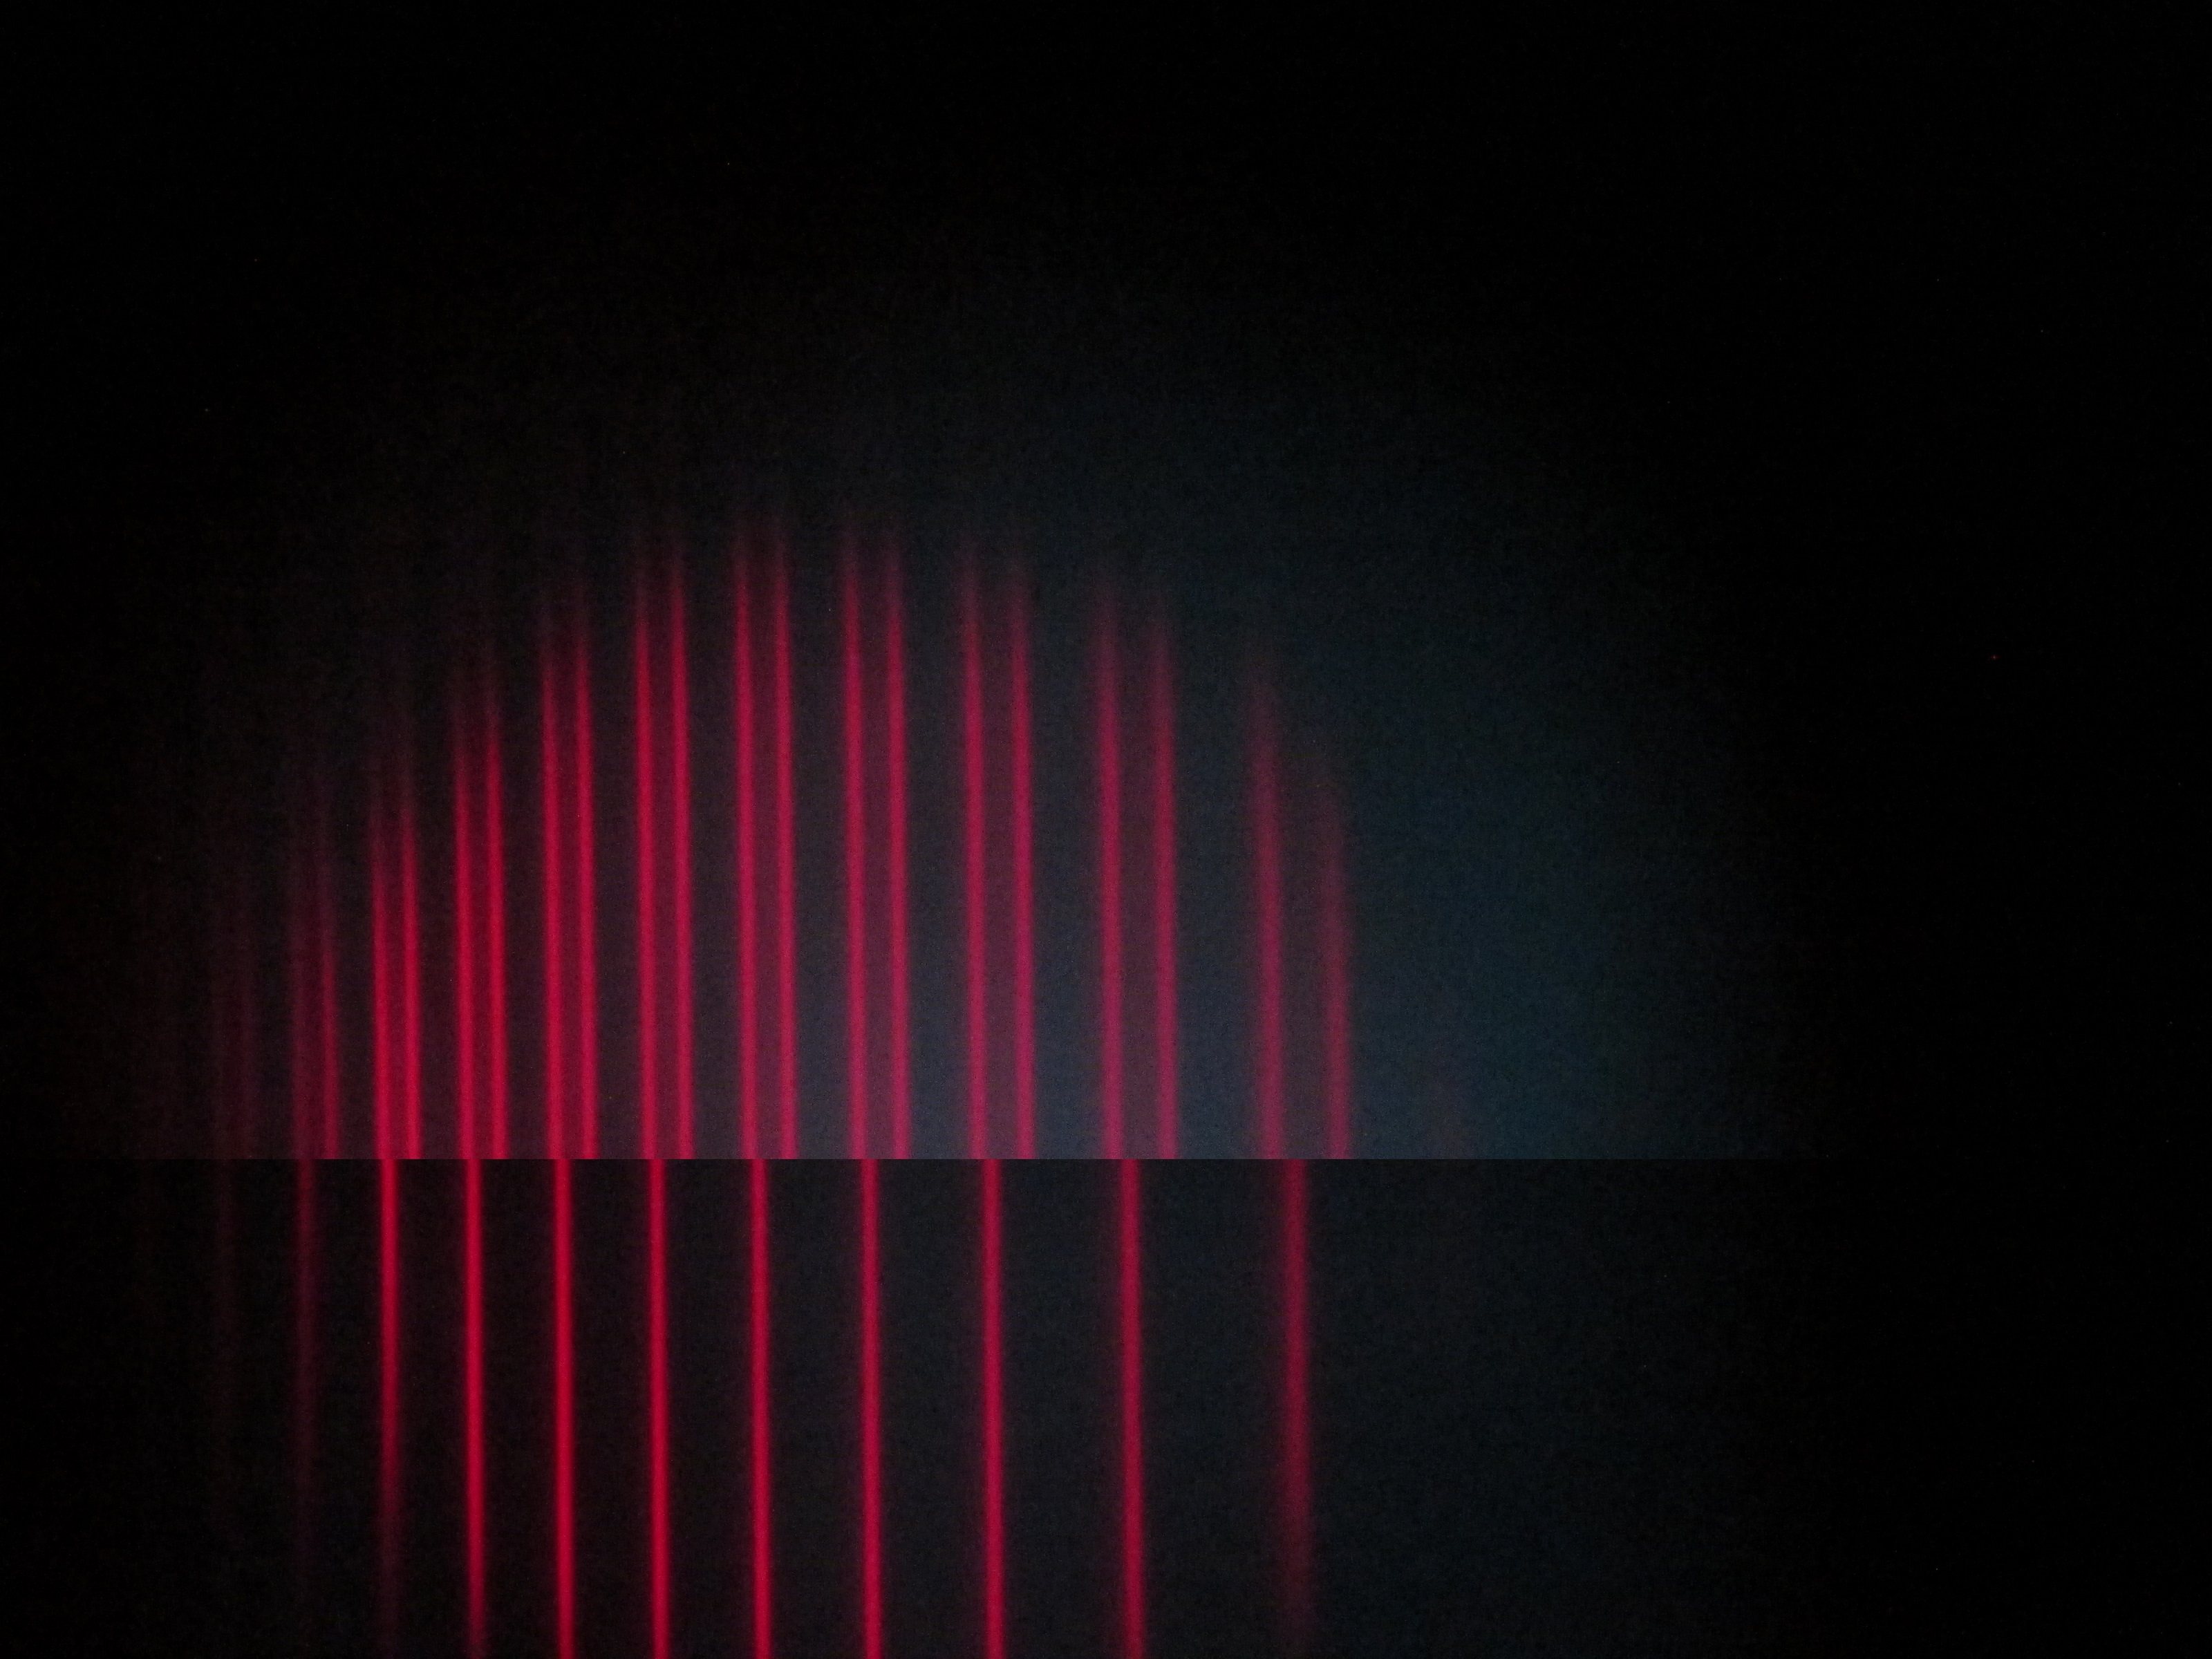
\includegraphics[width=0.75\textwidth]{content/data/Rot_0_sigma_uebernander.JPG}
    \caption{Im oberen Teil des Bilder ist das $\sigma -$Polarisierte Licht unter Einfluss des Zeeman-Effekts zu sehen. Im unteren Teil ist die rote Spektrallinie der Lampe ohne Magnetfeld eingeblendet.}
    \label{fig:rot-sigma}
\end{figure}

Es werden die Werte $\Delta s$ und $\delta s$ bestimmt diese sind in \autoref{tab:sigma-rot} zu sehen.
Zudem sind die Messwerte garphisch in \autoref{subfig:Rot_mess} zu sehen.
In der linken \autoref{subfig:Rot_mess} sind die Messwerte $\Delta s$ und $\delta s$ gegen die Ordnung aufgetragen,
in der rechten \autoref{subfig:Rot_versch} sind die berechneten Wellenlängenverschiebung zu sehen.
\begin{table}
    \centering
    \caption{$\Delta s$ der roten Spektrallinie und $\delta s$ des $\sigma -$Polarisiertem Lichts.}
    \begin{tabular}{cccc}
        \toprule
        Ordnung & $\Delta s \, /$ Pixel & $\delta s \, /$ Pixel & $\delta \lambda \, / \, \si{\nano\meter}$ \\
        \midrule
        1   &   308  &    76 & $\SI{0.00603(40)}{}$   \\
        2   &   244  &    63 & $\SI{0.00631(51)}{}$   \\
        3   &   228  &    59 & $\SI{0.00632(55)}{}$   \\
        4   &   202  &    59 & $\SI{0.00714(63)}{}$   \\
        5   &   190  &    42 & $\SI{0.00540(65)}{}$   \\
        6   &   177  &    40 & $\SI{0.00552(70)}{}$   \\
        7   &   168  &    34 & $\SI{0.00494(74)}{}$   \\
        8   &   164  &    29 & $\SI{0.00432(75)}{}$   \\
        9   &   147  &    21 & $\SI{0.00349(84)}{}$   \\
        10  &   168  &    21 & $\SI{0.00305(73)}{}$   \\
        \bottomrule
    \end{tabular}
    \label{tab:sigma-rot}
\end{table}

\begin{figure}
    \caption{Links die Messwerte $\Delta s$ und $\delta s$ gegen die Ordnung geplottet und rechts die berechnete Wellenlängenverschiebung gegen die Ordnung aufgetragen.}
    \begin{subfigure}{0.48\textwidth}
        \centering
        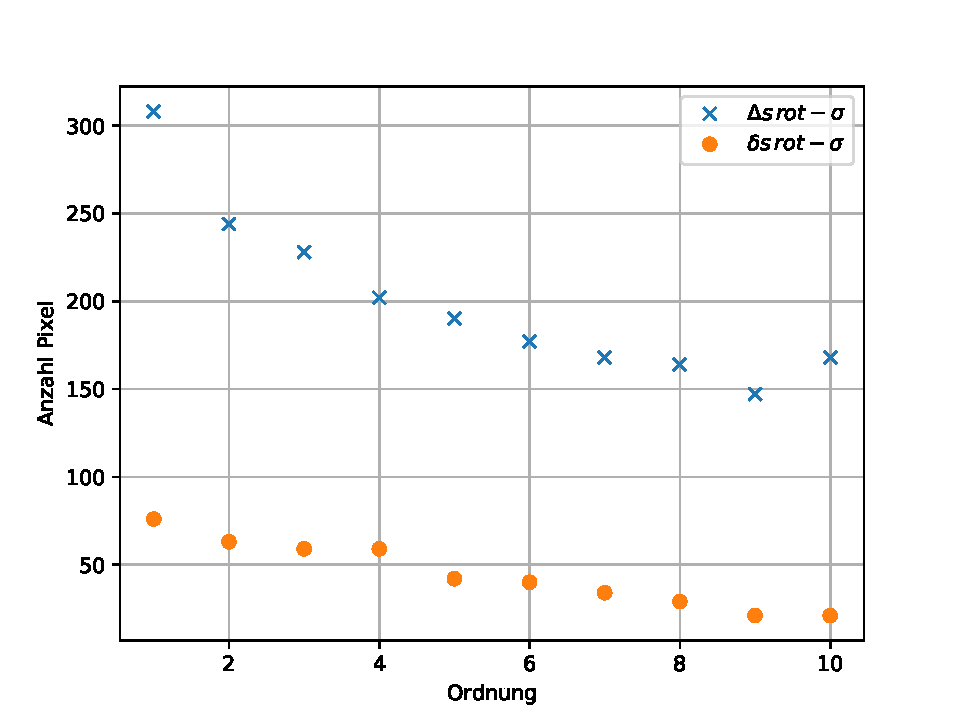
\includegraphics[height=5cm]{content/data/Rot_messwerte.pdf}
        \caption{Messwerte $\Delta s$ und $\delta s$ in Anzahl von Pixeln gegen die Ordnung aufgetragen.}
        \label{subfig:Rot_mess}
    \end{subfigure}
    \hfill
    \begin{subfigure}{0.48\textwidth}
        \centering
        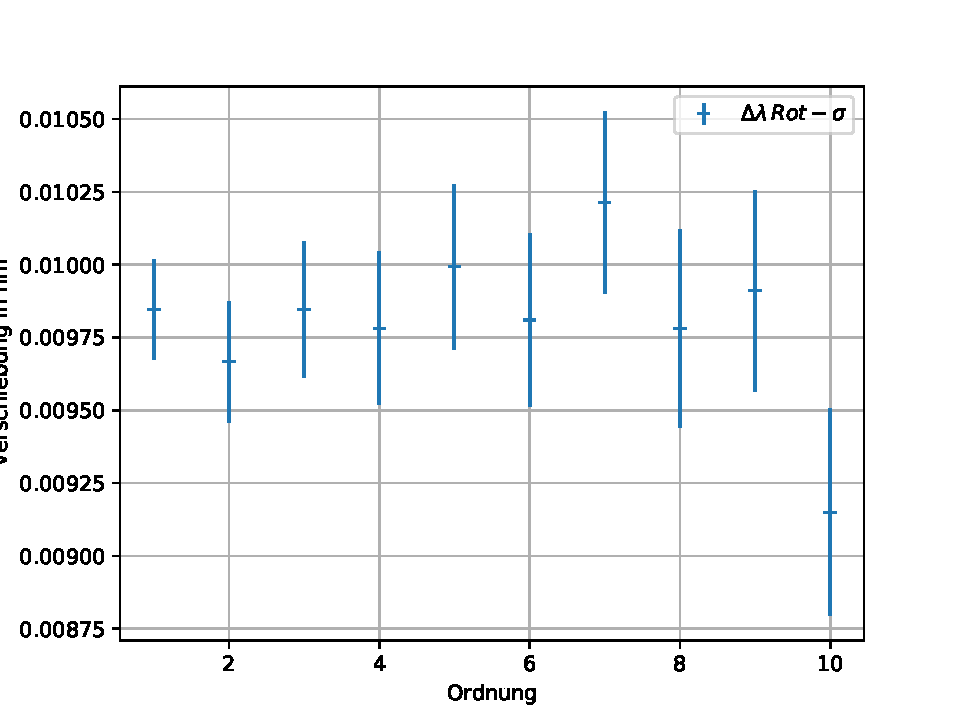
\includegraphics[height=5cm]{content/data/Rot_verschiebung.pdf}
        \caption{Die berechnete Wellenlängenverschiebung in $\si{\nano\meter}$ in Abhängigkeit von der Ordnung.}
        \label{subfig:Rot_versch}
    \end{subfigure}
    \label{fig:Rot_mess_versch}
\end{figure}
\FloatBarrier
Aus den Werten der \autoref{tab:sigma-rot} wird nach Gleichung \eqref{eq:Wellenlaengenverschiebung} die Wellenlängenverschiebung berechnet.
Danach wird über alle Werte gemittelt.
Es wird ein systematischer Fehler von $\pm 5$ Pixeln angenommen.
Die Wellenlängenverschiebung für die rote $\sigma -$Polarisierte Linie beträgt
\begin{align*}
    \delta \lambda _\text{$\sigma$-rot} =&  \SI{0.00544(020)}{\nano\meter} \, . \\
\end{align*}
\FloatBarrier
Alle gemittelten Wellenlängenverschiebungen sind nocheinmal in \autoref{tab:Wellenlaengenverschiebung_alle} zusammengefasst.

\begin{table}
    \centering
    \caption{Die gemittelten Wellenlängenverschiebung für das blaue $\pi$- und $\sigma$- Polarisierte, sowie rote $\sigma$- Polarisierte Licht unter Einfluss des Zeeman Effekts.}
    \begin{tabular}{cc}
        \midrule
        $\delta \lambda _\text{$\pi$-blau}$ &= $\SI{0.00316(011)}{\nano\meter}$ \\
        $\delta \lambda _\text{$\sigma$ -blau}$ &= $\SI{0.00621(012)}{\nano\meter}$ \\
        $\delta \lambda _\text{$\sigma$-rot}$ &=  $\SI{0.00544(020)}{\nano\meter}$ \\
        \bottomrule
    \end{tabular}
    \label{tab:Wellenlaengenverschiebung_alle}
\end{table}

\subsection{Berechung der Landé-Faktoren}

Zur Berechnung der Landé-Faktoren der verschiedenen Spektrallinien, wird die Gleichung \eqref{eq:Lande_Faktor} genutzt.
Es werden die gemittelten Wellenlängenverschiebungen aus \autoref{tab:Wellenlaengenverschiebung_alle} verwendet um die Landé-Faktoren zu berechnen.
Der Fehler des Landé-Faktors wird nach
\begin{equation*}
    F(g_\text{ij}) = \frac{hc}{\lambda^2 \mu _\text{B}} \sqrt{\left ( \frac{1}{B} F(\delta \lambda) \right)^2}
\end{equation*}
bestimmt.

Die berechneten Landé-Faktoren sind in \autoref{tab:Lande-Faktor} zu finden.
Zu den jeweiligen Landé-Faktoren sind dort auch die genutzten $B$-Felder, die Polarisierungen und Wellenlängen der Spektrallinien zu sehen.

\begin{table}
    \centering
    \caption{Die berechneten Landé-Faktoren, sowie die Art der Polisierung und die Wellenlänge des genutzten Lichts.}
    \begin{tabular}{cccc}
        \toprule
        $\lambda / \si{\nano\meter}$ & Polarisierung & $B / \si{\milli\tesla}$ & Landé-Faktor \\
        \midrule
        480.0 & $\pi$ & 443 & $\SI{0.672(25)}{}$ \\
        480.0 & $\sigma$ & 365 & $\SI{1.540(33)}{}$ \\
        643.8 & $\sigma$ & 443 & $\SI{0.613(25)}{}$ \\
        \bottomrule
    \end{tabular}
    \label{tab:Lande-Faktor}
\end{table}

